\documentclass{amsart}
\usepackage{amsmath, amsthm, amssymb, amscd}
\usepackage{color}
\usepackage{tikz-cd}
\usetikzlibrary{shapes.geometric}

\begin{document}

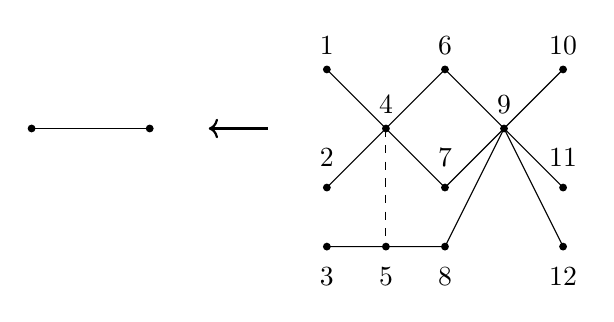
\begin{tikzpicture}[scale=0.75]
\draw (-6,0)--(-4,0);
\draw[<-,thick] (-3,0)--(-2,0);

\draw (-1,-1)--(0,0)--(1,1)--(2,0)--(3,1);
\draw (0,0)--(1,-1)--(2,0);
\draw (-1,1)--(0,0);
\draw (2,0)--(3,-1);
\draw (-1,-2)--(0,-2)--(1,-2)--(2,0)--(3,-2);
\draw[dashed] (0,0)--(0,-2);

\foreach \q in {(-6,0),(-4,0),(-1,1),(-1,-1),(0,0),(1,1),(1,-1),(2,0),(3,1),(3,-1),(-1,-2),(0,-2),(1,-2),(3,-2)}
\node at \q [circle,fill,inner sep=1pt]{};

\node at (-1,1.4) {1};
\node at (-1,-0.5) {2};
\node at (-1,-2.5) {3};
\node at (0,0.4) {4};
\node at (0,-2.5) {5};
\node at (1,1.4) {6};
\node at (1,-0.5) {7};
\node at (1,-2.5) {8};
\node at (2,0.4) {9};
\node at (3,1.4) {10};
\node at (3,-0.5) {11};
\node at (3,-2.5) {12};
\end{tikzpicture}

\end{document}